\begin{center}
	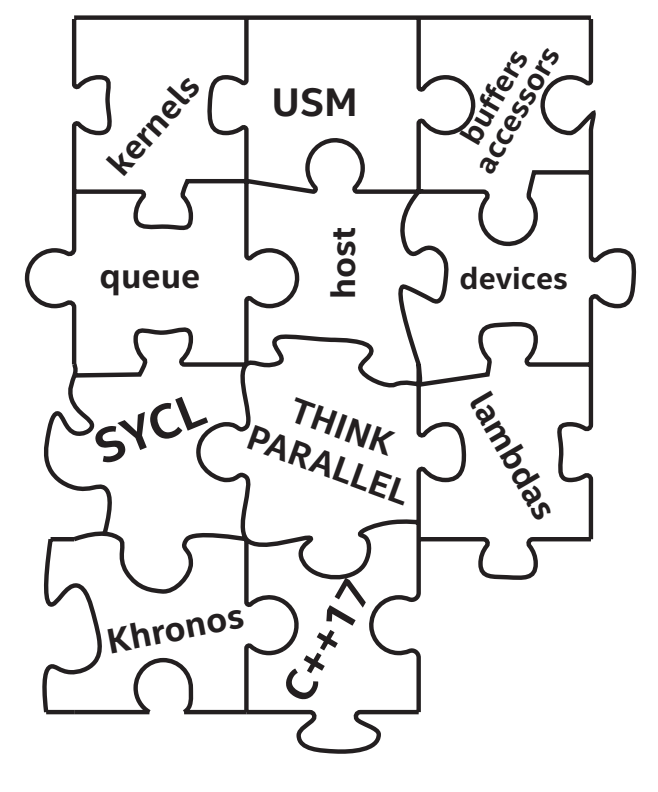
\includegraphics[width=0.5\textwidth]{content/chapter-4/images/1}
\end{center}

现在可以把第一批拼图拼在一起了。了解了如何在设备上执行代码(第2章)和数据(第3章)——现在必须做的就是如何处理它们。为了达到这个目的,现在补充一些容易忽略的东西。本章标志着从教学示例向实际并行代码的转变,会扩展前面章节中的代码示例的细节。\par

用一种新的并行语言编写第一个程序似乎很困难,特别是对并行编程的新手。语言规范不是为应用程序开发人员编写的,通常需要对术语有所了解:\par

\begin{itemize}
	\item 为什么会有不止一种表达并行性的方法?
	\item 应该用哪种方法来表达并行性?
	\item 关于执行模型,需要了解多少?
\end{itemize}

本章会解决这些问题和其他问题。我们会了解数据并行内核的概念,使用工作代码示例讨论不同内核形式的优缺点,并重点介绍内核执行模型。\par







